\documentclass[runningheads]{llncs}
\usepackage{graphicx}
\usepackage{times}
\usepackage{float}
\usepackage{latexsym}
\usepackage[T1]{fontenc}
\usepackage[utf8]{inputenc}
\usepackage{microtype}
\usepackage[utf8]{inputenc}
\usepackage[ruled,vlined]{algorithm2e}
\graphicspath{ {./images/} }
\begin{document}
\title{Neural Network Pruning as a N Player NIM Game}
\author{Daniel Campos\orcidID{0000-0002-5138-8426} }
\authorrunning{D. Campos et al.}
\institute{University of Illinois at Urbana-Champaign, Urbana, Il, 61801, USA}
\maketitle              % typeset the header of the contribution
%
\begin{abstract}
Unstructured pruning has become one of the most popular methods for Neural Network model pruning since it provides an intuitive method of extracting a sub network from the original Neural Network which matches the pruning goals. Pruning approaches have been used to reduce model size, increase adversarial robustness, increase stability and generizability, and increase model inference speed but each of these goals works independently. By framing Network Pruning as a $N$ player NIM game we provide a framework which can be used to combine pruning strategies depending on needs. In our work, each pruning method takes the role of a NIM game player where they remove weights from a network in an iterative fashion. We find that 2 player methods combining $L1$ and Random pruning outperform existing method across datasets and models. We believe this formulation of network pruning provides a comprehensive framework which can be used to prune networks for multiple goals. 
\keywords{Neural Network \and Subtraction Game \and Neural Network Pruning.}
\end{abstract}
\section{Introduction}
Neural Networks have become popular choices for complex computation tasks like image recognition \cite{Howard2017MobileNetsEC}, image generation \cite{Goodfellow2014GenerativeAN}, speech processing \cite{Zhao2017RecurrentCN}, and question answering \cite{Seo2017BidirectionalAF}. These networks have grown to hundred billions of parameters \cite{Brown2020LanguageMA} which require specialized hardware like clusters of GPUs and FPGAs in order to infer on unseen data. Recent work has shown that larger networks can learn quicker \cite{Li2020TrainLT}, are more accurate and are more sample efficient \cite{Kaplan2020ScalingLF}. Seeking to allow the improvements that large models have brought to be used on smaller devices and in a more energy efficient way researchers have produced many methods which produce smaller networks that approximate, match, or exceed the original network performance. \\ 
Model distillation, quantization, and pruning have emerged as successful methods to produce smaller networks from the original over-parametized network. In model distillation  \cite{Ba2014DoDN} the original network is used to train a smaller network to mimic the behavior of the large network. In model quantization \cite{Han2016DeepCC} models are made smaller by  reducing the numbers of bits that represent each weight. Model Pruning \cite{LeCun1989OptimalBD} has focused on finding sub-networks in the original network by structured and unstructured pruning. In structured pruning, successful sub-networks are found by removing neurons  \cite{Wang2019StructuredPF} or larger network specific structures like attention heads \cite{Voita2019AnalyzingMS}. In unstructured pruning the successful sub-networks are found by setting individual weights to zero \cite{Kwon2019StructuredCB}. \\
Using network pruning, The Lottery Ticket Hypothesis \cite{Frankle2019TheLT} proved the concept that in large neural networks there exists a sub network which can match the accuracy of the full network despite its smaller size. Building on the notion that there are many sub networks in an overparamertized network we formulate network pruning as a combinatorial problem. Given an initial structure $S$ and a target network size $\epsilon$ the goal is to find the sub network $s_m$ of size $\epsilon$ which maximizes the optimization metric. Sub networks can have many different optimization goals such as: accuracy, size, adversarial robustness, computation speed, explainability, etc. Given that networks commonly have millions of parameters and the network can continually be updated by retraining even a greedy strategy for optimal model selection would require a millions of combinations. Instead, using network pruning we can can produce sub network $s_a$ with minimal compute and using a targeted pruning strategy we only remove neurons that minimize our optimization goal. \\
Believing that the future of network pruning is likely to focus on multi metric optimization we formulate network pruning as a $N$ player game of NIM. In a game of NIM \cite{Dass2006SecretsBT} players remove items from a variety of bins in alternating turns. Using this strategy we are able to combine different pruning strategies to produce networks that maximize sparsity and performance and outperform traditional iterative pruning mechanisms. 
\section{Related Work}
Neural network compression is an area that has attracted the attention of researchers for the last few decades. Methods for producing smaller networks that approximate original network performance include: distillation, quantization, structured and unstructured pruning. While each of these methods can compress models substantially on their own many researchers have found that some combination of these methods can produce the smallest models with the highest performance \cite{Polino2018ModelCV}, \cite{Sanh2020MovementPA}. \\
Model distillation \cite{Ba2014DoDN} addresses compressing models by first training a large network and calling it a teacher. Then using this teacher model a smaller student model learns to approximate what the teacher model would do. This framework is quite popular because it can leverage existing large models easily and the student model can be designed to fit the application requirements in terms of speed and model size. Distillation has been one of the most common methods of deployment of large scale language models where student models like DistilBERT \cite{Sanh2019DistilBERTAD} can approximate full model performance at a fraction of the size. \\
Model quantization \cite{Gong2014CompressingDC} \cite{Han2016DeepCC} addresses compressing models by reducing the number of bits that are require to represent parameters in a model. In simple implementations this means changing representation of weights from Float32 to float16(effectively cutting model size in half). Complex implementations tune networks to find the smallest amount of bits that can be used for weights, biases, and gradient updates using values as low as 1 bit \cite{Courbariaux2016BinarizedNN}. Quantization is particularly effective because it both leverages that networks are defaulted to a level of precision which is too high and by decreasing the size of representations networks are forced to share weights making networks more robust. \\
Model pruning \cite{LeCun1989OptimalBD} addresses model compression by decreasing the connection in a network. The goal of network pruning is to produce a sub network of the original network which optimizes some network property(accuracy, speed, robustness) while preserving the original network function. Network pruning has been show to produce a similar effect to random noise injection \cite{Bartoldson2019TheGT} and this noise can be used to make the network more efficient. Bartoldson et al., showed that network pruning is not just used for decreasing size but can be used to increase the generalization of the network. The formulate that pruning methods generally generally focus on how important a prune target is currently to the network but believe that algorithms should also should be designed to consider the damage that removal has on a network.  \\
As mentioned earlier, there is structured pruning and unstructured pruning. In structured pruning, the structure of the network is altered by removal of entire neurons, layers, or portions neural network. This method has proven especially successful in language model compression where despite having dozens of attention heads \cite{Vaswani2017AttentionIA} few heads do most of the work and the rest can be removed \cite{Michel2019AreSH}. In unstructured pruning the network structure is altered by removal of individual weights. Unstructured pruning when paired with optimization engines can produce networks that are smaller, more accurate, and run faster than the original network. \\
Liu et al., \cite{Liu2019RethinkingTV} proposed that network pruning is doing something similair to neural architecture search to find an optimal architecture given a set of optimization metrics. Recently, researchers have explored pruning methods that simultaneously remove and reintroduce weights \cite{Jia2020StochasticMP} which helps keep a pruned network from being stuck in a local minimum. Within unstructured pruning methods can be local or global. Global pruning pools together all parameters across layers while local performs each pruning operation focused on individual layers. \\
The use of Game Theory has proven successful for model compresion. KDGAN \cite{Wang2018KDGANKD} explores formulation of distillation as a 3 player game which
improves model performance, train time, and training efficient. Many more
methods \cite{Guo2018SparseDW} \cite{Dhillon2018StochasticAP}, \cite{Sehwag2020OnPA}, \cite{Xie2020BlindAP}, explore the use of Adversarial methods in model
pruning with a goal of making NN more robust to adversarial inputs. HYDRA \cite{Sehwag2020HYDRAPA} prunes models for adversarial robustness by formulating pruning as a empirical risk minimization (ERM) problem removing neurons that maximize risk.
\section{Pruning as an N Player Game}
We propose the formulation of pruning as an $N$ player game of NIM as a way to allow multi objective network pruning. NIM is traditionally a combinatorial game where two players take turns removing objects from several heaps. NIM is the most well known example of an impartial game because every player has the same amount of moves in a game. In our implementation, the game is played on unstructured local pruning where each player is able to remove a single weights from the layer of the neural network which is currently being played. This game is an extensive subtraction game since it happen over many rounds of play and players make moves by removing parts of a structure. \\
In this game, pruning methods are implemented as a collection of $P$ players in which each player $p \in P$ has a unique strategy which does does not change based on other players nor any prior round. Prior to playing their turn, each player ranks the existing weights based on how each weight maximizes their optimization metric. When its a players turn to play they simply select the first non zero weight in their ranking. At the beginning of each round the order in which the players $p \in P$ execute their prune is selected at random to ensure that one method is not favored over others.  Since the outcome of the game is independent of players performance we will not discuss their reward and utility functions further. \\
The utility in this implementation of pruning is the ability to easily combine strategies and ratio of strategies depending on targeted applications. In single objective pruning there is only one player who plays the game alone. As more optimization goals get introduced the amount of players grow. In a complex game there may be multiple players with the same strategy which gives the game organizer(the network pruner) the ability to set importance of pruning optimization metrics. 
\section{Experiment}
The structure of our experiments is straightforward: train an initial baseline method and prune this networks iteratively using each of the candidate methodologies. To evaluate the effect of our formulation we select 3 popular image recognition frameworks which vary in structure, size and recency: VGG-16 \cite{Simonyan2015VeryDC}, ResNet50 \cite{He2016DeepRL}, DPN92 \cite{Chen2017DualPN}. We train each network on the CIFAR-10 \cite{Krizhevsky2009LearningML} and CIFAR-100 \cite{CIFAR-10} dataset which are common benchmarks for evaluating image systems. The CIFAR-10 dataset consists of 60,000 32x32 color images where each image belongs to one of ten classes. The CIFAR-100 dataset is just like CIFAR-10 but it has 100 classes instead of 10 and each class includes 600 examples instead of 6,000.
\subsection{Generating Baselines}
Each of our model baselines are trained in an identical fashion. For each combination of model architecture and dataset each model is trained with a batch size of 128, an initial learning rate of 0.1 and trained for 1000 epochs. Models are trained using 2 Nvidia 2080 Ti GPUs with a  Intel Core™ i9-10900X CPU and 128GB of RAM. Training time ranges from 1 hour for VGG-16 to 1 day for DPN-92. During this training regime we evaluate the model on the validation portion of the dataset at the end of each epoch and the final candidate baseline is the checkpoint that maximised validation accuracy. Numerical details on baseline models can be found in Table \ref{tab:tab1}.
\subsection{Pruning}
Our pruning experiments are focused on Iterative Pruning as it has become one of the most popular methods. In these experiments we only prune the weights of convolutions layers and we prune each layer independently. While other research has shown that optimal pruning of a network has different sparsity at different layers \cite{Blalock2020WhatIT} we keep a uniform pruning for ease of experimentation. By focusing only on pruning convolutional layers we are not exploring every possible sub network but as shown in Table \ref{tab:tab1}, convolutional weights make up the majority of each network. The process is formalized in Algorithm 1 where $NN$ is a neural network, $lambda_i$ is the $i$th prunable layer in a $NN$, $\pi$ represents what percentage of weights need to be trimmed at each time step and $M$ represents a sorting function which maximizes the pruning optimization metric, $P$ represents the players playing our NIM game where each player $p_i$ has a strategy $s_i$ which is based on a $m_i$, $s_j$ represents sparsity at epoch j and $s_{target}$ represents the target network sparsity. \\
In our experiments we set $s_{target} = 0.95$, $\pi=0.05$ and we evaluate model performance after each epoch. Our iterative pruning has three steps: stabilization, pruning, and fine tuning. In stabilization the network is trained with a learning rate of $0.1$ for 2 epochs. In network pruning we gradually remove $\pi\%$ of  weights and retrain the network with one pass the entire training data with a learning rate of 0.01. This stage lasts 19 epochs as $s_j = s_{j-1} + \pi$ takes 19 steps to reach $s_{target}$. In fine tuning we set the learning rate to 0.001 and train the network for 10 epochs on the full dataset to ensure the network has reached optimal performance and is stable. \\
In the network pruning step, we prune each layer independently and implement it as a NIM game as shown in Algorithm 2. In this NIM game there are some set of players $N$ which each has a strategy for network pruning $s_i$. For each round, player order is randomly selected and each players removes a single weight from the layer. A NIM game is played for each $\lambda_i \in NN$ and if the network sparsity is under the $s_{current sparsity}$ then another round of NIM is played on each layer that is still under the target. Since target sparsity is a global parameter some layer sparsity will have lower and higher sparsity than the target. If a layer is over pruned in one epoch it will not be pruned until its sparsity is lower than the target.  Each player $n_i \in N$ is defined by what pruning strategy is used and while our experiments focus on 2 and 3 player games $N$ could be much bigger. We will expand on network pruning as an $N$ payer game shortly.
\subsection{Pruning Methods}
Using the methodology previously described we explore the effect of. To explore how NIM can be used in Network pruning we formulate 8 games with a mixture and strategies. Each method is implement as $1-n$ player game where each player has a strategy $s_i$ which is represented via a sorting method $M_i$ which they use to sort the weights $W$ of the given layer they are pruning. Each of these ranking methods ranks weights of 0 as lowest and then ranks all existing weights to maximize their desired outcome. Details on each pruning method can be founding in the appendix.
\section{Results}
In our experiments our main goal was to see if combining pruning strategies could lead to improved models across sparcity. If we focus initially on performance on high sparcity networks(90\% +) we find that L1 + Random pruning out performs other methods on five out of our six baselines. We believe this is because the combination of L1 and random pruning simultaneously keeps the most important sub networks while introducing generalization as the network cannot only rely on the strongest weights. We also note that across all experiments we see a large variation in optimal pruning mechanism given a target sparcity. We believe this further underscores the utility of the NIM game because it allows researchers to choose the most optimal game formulation depending on desired results. We also note that we see a wider spread in model accuracy on pruning of models targeting CIFAR-10 vs CIFAR-100. We believe this is because the dataset has few classes which results in more independent class specific sub networks which our various methods effect differently. \\
One of the surprises in our experiments was the consistent high performance of Random pruning even at high sparcity. We believe this is the case because even at high scarcities since the datasets are easier the networks are still highly over parametized. We reason that as we scale the difficulty of the target task random pruning alone would start to cause complete model failure. Since the focus of our work is on the formulation of pruning as a $N$ player game we will not further analyze our results but the full results can be found in the appendix. 
\section{Conclusion and Future Work}
The addition of game theory to AI has proven to be a robust framework which leads to new discoveries and methods. We connect this literature to Neural Network pruning to build a framework which can optimize networks to a variety of goals. Using this framework we then show that the combination of strategies can be used to surpass single strategy pruning mechanism across a wide and representative set of models. By using a game of NIM to prune a network we have created a framework which can be used to create pruning strategies which outperforms traditional iterative pruning with limited computational overhead. While our method shows promise on CIFAR-10 and CIFAR-100 we believe that larger and more complex datasets are required to explore the effects of our pruning strategies further. \\
Going forward we many areas we wish to continue to explore. First off, we wish to explore what other games can be used to model Neural Networks pruning. While we show that NIM can be used successfully to improve pruning we believe that there may be other game formulations which are a better fit. Second, we wish to explore how NIM pruning can be used in the pruning of large language models. These models have scaled to billions of parameters and are used for a breadth of tasks so multi goal pruning will likely prove beneficial. Third, we want to explore network performance with the addition of new pruning goals. We believe the addition of FLOP optimization, Adversarial Robustness, and class aware pruning can all be introduced to NIM pruning to produce networks that maximize many goals and are small. Finally, in future work we seek to improve our framework for pruning to allow for global weight pruning. By moving to global weight pruning the game can expand to have strategies which optimize to network depth and breath, weight distribution, and take into account the varying sensitivity to pruning each layer may have. 
\bibliographystyle{splncs04}
\bibliography{references}
\section{Appendix}
\subsection{Baseline Statistics}
\begin{tiny}
\begin{table}
\begin{tabular}{|l|l|l|l|l|}
\hline
Model& Data   & Param & Conv& Acc\\ \hline
VGG-16       & CIFAR-10  & 14.73             & 14.71   & 86.85                 \\ \hline
VGG-16       & CIFAR-100 & 14.77           & 14.71     & 58.43                 \\ \hline
RESNET50     & CIFAR-10  & 23.52  & 20.68              & 86.89              \\  \hline
RESNET50     & CIFAR-100 & 23.71 & 20.68               & 62.74               \\\hline
DPN-92       & CIFAR-10  & 34.24         & 29.88       & 88.61                 \\\hline
DPN-92       & CIFAR-100 & 34.47            & 29.88    & 66.13  \\  \hline             
\end{tabular}
\caption{Baseline models accuracy, characteristics, and parameter size. Parameters are in millions and Conv represents the parameters in convolutional layers. }
\label{tab:tab1}
\end{table}
\end{tiny}
\subsection{L1 Pruning Mechanism}
We implement L1 as a single player game where player $n_1$ sorts weights by ranking those closest to the L1-Norm as lowest. The L1-norm is the sum of the magnitudes of the vectors in a space. L1 pruning is thought to be a successful because weights with a small l1 are likely to produce small activation's and thus not influence the end result much.In most existing pruning implementation L1 pruning usually produces the best results. 
\subsubsection{Random Pruning Mechanism}
We implement Random as a single player game where player $n_1$ sorts weights at random. Random pruning has shown to be highly effective as it acts as a regularizer in the network forcing many sub networks to learn effective representations as the network cannot rely on only one part of the network.
\subsubsection{Magnitude Pruning Mechanism}
Magnitude pruning is a common strategy in which all weights closest to zero are removed. We implement this strategy as a two player game where the first player does positive magnitude pruning and the second does negative magnitude pruning. The positive pruning agent, $n_1$, sorts weights by ranking $w_j \in W$ where $w_j >= 0$ which removes smallest positive weights. The negative pruning agent, $n_2$, behaves the same as positive but removes the smallest negative weights.
\subsection{L1 + Random Pruning Mechanism}
We implement L1 + Random as a two player game where the first player, $n_1$, plays an L1 strategy and the second player, $n_2$, plays a random strategy. This strategies goal is to remove unimportant weights and force the existing network to learn a sparse generalizable representation.
\subsection{L1 + Magnitude Pruning Mechanism}
We implement L1 + Magnitude as a three player game where the first player, $n_1$, plays an L1 strategy, the second player, $n_2$, plays a positive magnitude strategy and the third player, $n_3$, plays a negative magnitude strategy.
\subsection{Random + Magnitude Pruning Mechanism}
We implement Random + Magnitude as a three player game where the first player, $n_1$, plays an random strategy, the second player, $n_2$, plays a positive magnitude strategy and the third player, $n_3$, plays a negative magnitude strategy.
\begin{tiny}
\begin{algorithm}[]
\label{algo:iterprune}
\SetAlgoLined
\KwResult{Sparse Neural Network}
\SetKwFunction{FPrune}{Prune}
\SetKwFunction{FMain}{IterativePrune}
\SetKwFunction{FTrain}{Train}
\SetKwFunction{FEval}{Evaluate}
\SetKwFunction{FNim}{NimGame}
\SetKwFunction{Fc}{isConvLayer}
\SetKwFunction{Fs}{GetNetworksparsity}
\SetKwFunction{Fss}{GetLayersparsity}
  \SetKwProg{Fn}{Function}{:}{}
  \Fn{\FMain{$NN, \pi, s_{target}, P$}}{
  pruningepochs = $\frac{s_{target}}{\pi}$\;
  \FEval($NN$)\;
  \For{i in range(0,2)}{
      \FTrain{$NN$}\;
      \FEval($NN$)\;
    }
    $s_{current target} = 0$\;
    \For{i in range(0,pruningepochs)}{
        $s_{current target} =  s_{current target} + \pi$ \;
        $s_{current} =$ \Fs{$NN$}\;
        \While{$s_{current} < s_{current target}$}{
            \For{$\lambda \in NN$}{
                \If{\Fc{$\lambda$}} {
                    \If{\Fss{$\lambda $}   $ < s_{current target}$} {
                        $\lambda = $ \FNim{$\lambda , P$}\;
                    }
                }
                $s_{current} =$ \Fs{$NN$}\;
        }
        }
        \FEval($NN$)\;
        \FTrain{$NN$}\;
        \FEval($NN$)\;
    }
    \For{i in range(0,10)}{
      \FTrain{$NN$}\;
      \FEval($NN$)\;
    }
}
\caption{Iterative Network Pruning}
\end{algorithm}
\end{tiny}
\begin{algorithm}[]
\label{algo:nim}
\SetAlgoLined
\KwResult{pruned layer of a NN}
\SetKwFunction{FPrune}{Prune}
\SetKwFunction{FMain}{NimGame}
\SetKwFunction{Fs}{getStrategy}
\S
  \SetKwProg{Fn}{Function}{:}{}
  \Fn{\FMain{$\lambda_i, P$}}{
  \For{p $\in$ P}{$\lambda_i$=
  \FPrune{$\lambda_i$,\Fs{$p$}}\; 
  }
}
\caption{Iterative Network Pruning}
\end{algorithm}
\begin{algorithm}[]
\label{algo:prune}
\SetAlgoLined
\KwResult{Pruned Neural Network Layer}
\SetKwFunction{FMain}{Prune}
  \SetKwProg{Fn}{Function}{:}{}
  \Fn{\FMain{$\lambda_i$, $M$}}{
        idx-sort = Sort weights $w_j \in \lambda_i$ using by $M$ \CommentSty{//produce a sorted lookup index of weights in layer based on a sorting function $M$}\;
        j = 0 \; 
        \While{$\lambda_i$[idx-sort[j]] == 0} {
         j = j + 1  \CommentSty{//Find first non pruned weight}
        }
        $\lambda_i$[idx-sort[j]] = 0 \CommentSty{Prune weight by setting to 0} \; 
        \KwRet $\lambda_i$
}
\caption{Prune Function sorts the weights in layer given using the optimization goal and sets the least important non zero weigth to 0 }
\end{algorithm}
\begin{figure}[H]
\centering
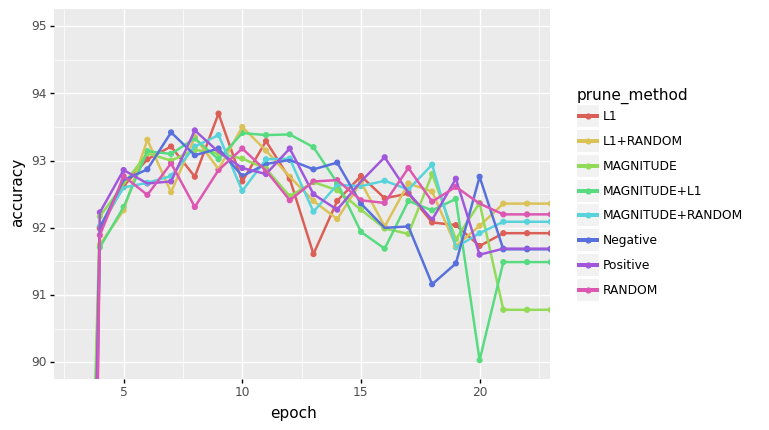
\includegraphics[width=6cm, height=6cm]{Paper/images/resnet50cifar10.png}
\caption{RESNET50 on CIFAR10}
\end{figure}
\begin{figure}[H]
\centering
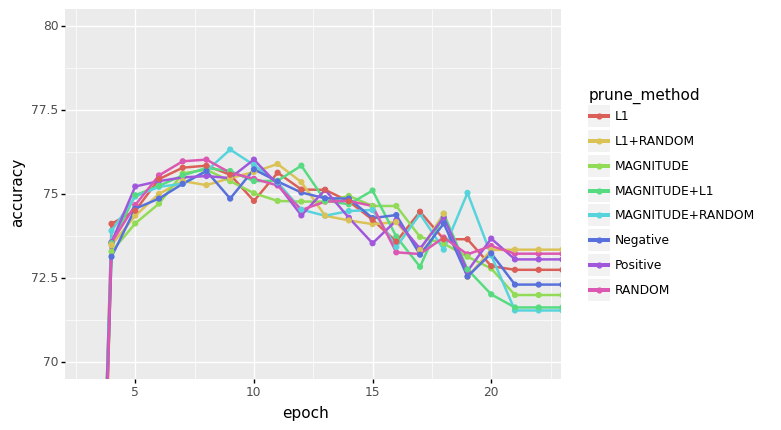
\includegraphics[width=6cm, height=6cm]{Paper/images/resnet50cifar100.png}
\caption{RESNET50 on CIFAR100}
\end{figure}
\begin{figure}[H]
\centering
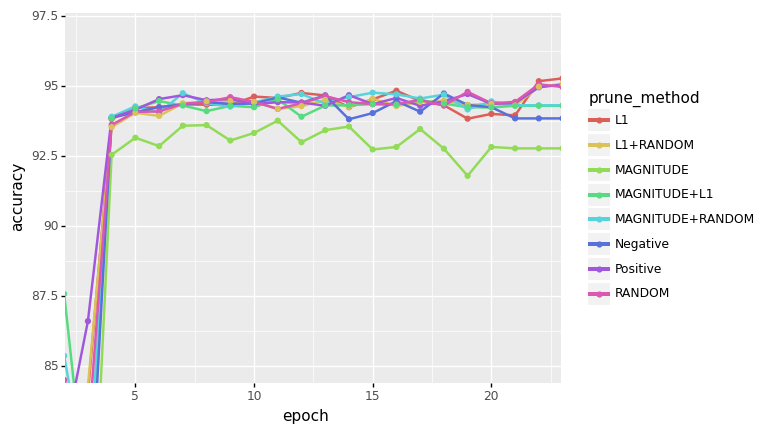
\includegraphics[width=6cm, height=6cm]{Paper/images/dpn92cifar10.png}
\caption{DPN92 on CIFAR10}
\end{figure}
\begin{figure}[H]
\centering
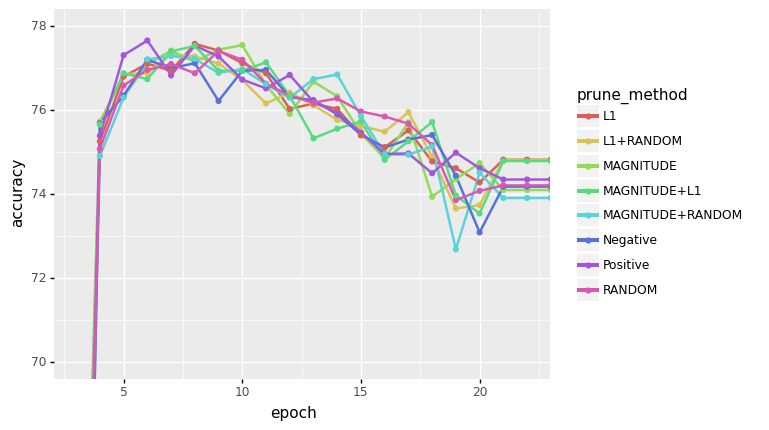
\includegraphics[width=6cm, height=6cm]{Paper/images/dpn92cifar100.png}
\caption{DPN92 on CIFAR100}
\end{figure}
\begin{figure}[H]
\centering
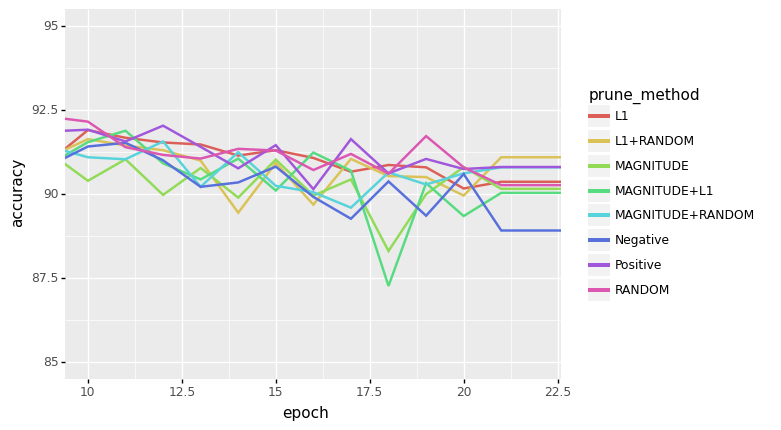
\includegraphics[width=6cm, height=6cm]{Paper/images/vgg16cifar10.png}
\caption{VGG16 on CIFAR10}
\end{figure}
\begin{figure}[H]
\centering
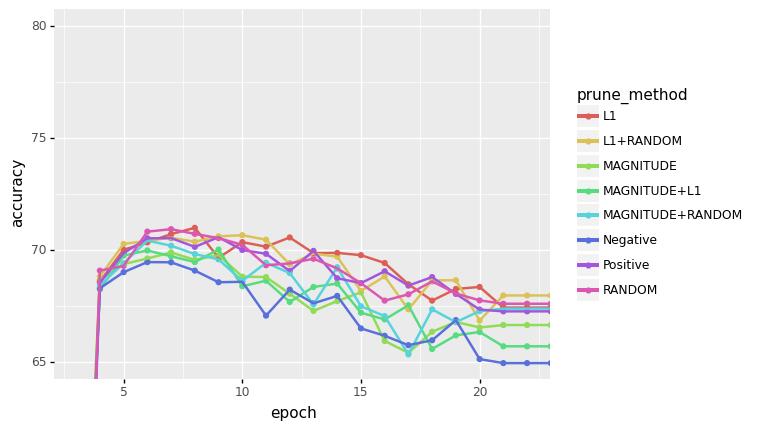
\includegraphics[width=6cm, height=6cm]{Paper/images/vgg16cifar100.png}
\caption{VGG16 on CIFAR100}
\end{figure}
\begin{table}[h]
\begin{tabular}{|l|r|r|r|}
\hline
     prune\_method &  sparsity &  accuracy \\ \hline
     Baseline  &  0.000000 &     66.13 \\ \hline
        MAGNITUDE &  0.925926 &     74.10 \\ \hline
        L1+RANDOM &  0.925926 &     74.82 \\ \hline
         Negative &  0.925926 &     74.18 \\ \hline
         Positive &  0.925926 &     74.35 \\ \hline
               L1 &  0.925926 &     74.82 \\ \hline
           RANDOM &  0.925926 &     74.21 \\ \hline
 MAGNITUDE+RANDOM &  0.925926 &     73.91 \\ \hline
     MAGNITUDE+L1 &  0.925926 &     74.79 \\ \hline
\end{tabular}
\label{tab:cifar100-DPN92}
\caption{DPN-92 on CIFAR 100. }
\end{table}


\begin{table}[h]
\begin{tabular}{|l|r|r|r|}
\hline
     prune\_method &  sparsity &  accuracy \\ \hline
   Baseline  &  0.000000 &     88.61 \\ \hline
               L1 &  0.925926 &     95.45 \\ \hline
         Positive &  0.925926 &     95.25 \\ \hline
         Negative &  0.925926 &     93.85 \\ \hline
 MAGNITUDE+RANDOM &  0.925926 &     94.32 \\ \hline
        MAGNITUDE &  0.925926 &     92.78 \\ \hline
           RANDOM &  0.925926 &     95.17 \\ \hline
        L1+RANDOM &  0.925926 &     95.16 \\ \hline
     MAGNITUDE+L1 &  0.925926 &     94.30 \\ \hline 
\end{tabular}
\label{tab:cifar10-DPN92}
\caption{DPN-92 on CIFAR 10. Unlike all other experiments the most successful mechanism is a one player game.}
\end{table}

\begin{table}[h]
\begin{tabular}{|l|r|r|r|}
\hline
     prune\_method &  sparsity &  accuracy \\ \hline 
     Baseline &  0.000000 &     86.85 \\ \hline
         Positive &  0.961008 &     90.81 \\ \hline
        MAGNITUDE &  0.985989 &     90.16 \\ \hline
         Negative &  0.961008 &     88.92 \\ \hline
           RANDOM &  0.975409 &     90.27 \\ \hline
 MAGNITUDE+RANDOM &  0.994909 &     90.80 \\ \hline
        L1+RANDOM &  0.981350 &     91.10 \\ \hline
               L1 &  0.975409 &     90.37 \\ \hline
     MAGNITUDE+L1 &  0.921536 &     90.04 \\ \hline
\end{tabular}
\label{tab:cifar10-VGG16}
\caption{VGG16 on CIFAR 10. While all methods outperform initial baseline the combination of L1+Random outperforms all other methods.}
\end{table}

\begin{table}[h]
\begin{tabular}{|l|r|r|r|}
\hline
     prune\_method &  sparsity &  accuracy \\ \hline 
        Baseline &  0.000000 &     58.43 \\ \hline
         Positive &  0.961008 &     67.27 \\ \hline
           RANDOM &  0.975409 &     67.61 \\ \hline
     MAGNITUDE+L1 &  0.921484 &     65.71 \\ \hline
        MAGNITUDE &  0.985989 &     66.66 \\ \hline
        L1+RANDOM &  0.981350 &     67.98 \\ \hline
         Negative &  0.961008 &     64.96 \\ \hline
 MAGNITUDE+RANDOM &  0.994906 &     67.39 \\ \hline
               L1 &  0.975409 &     67.44 \\ \hline
\end{tabular}
\label{tab:cifar100-VGG16}
\caption{VGG16 on CIFAR 100. While all methods outperform initial baseline the combination of L1+Random outperforms all other methods.}
\end{table}

\begin{table}[h]
\begin{tabular}{|l|r|r|r|}
\hline
     prune\_method &  sparsity &  accuracy \\ \hline
           Baseline &  0.000000 &     62.74 \\ \hline
           RANDOM &  0.925926 &     73.23 \\ \hline
         Positive &  0.925926 &     73.06 \\ \hline
        MAGNITUDE &  0.925926 &     72.00 \\ \hline
 MAGNITUDE+RANDOM &  0.925926 &     71.54 \\ \hline
     MAGNITUDE+L1 &  0.925926 &     71.63 \\ \hline
        L1+RANDOM &  0.925926 &     73.35 \\ \hline
         Negative &  0.925926 &     72.31 \\ \hline
               L1 &  0.925926 &     72.75 \\ \hline
\end{tabular}
\label{tab:cifar100-RESNET50}
\caption{RESNET50 on CIFAR 100. While all methods outperform initial baseline the combination of L1+Random outperforms all other methods.}
\end{table}

\begin{table}[h]
\begin{tabular}{|l|r|r|r|}
\hline
     prune\_method &  sparsity &  accuracy \\ \hline
         Baseline &  0.000000 &     86.89 \\ \hline
         Positive &  0.925926 &     91.69 \\ \hline
         Negative &  0.925926 &     91.68 \\ \hline
 MAGNITUDE+RANDOM &  0.925926 &     92.09 \\ \hline
        MAGNITUDE &  0.925926 &     90.78 \\ \hline
        L1+RANDOM &  0.925926 &     92.36 \\ \hline
               L1 &  0.925926 &     91.92 \\ \hline
           RANDOM &  0.925926 &     92.20 \\ \hline
     MAGNITUDE+L1 &  0.925926  &     91.49 \\ \hline
\end{tabular}
\label{tab:cifar10-RESNET50}
\caption{RESNET50 on CIFAR 10. While all methods outperform initial baseline the combination of L1+Random outperforms all other methods.}
\end{table}
\end{document}
